\documentclass[review]{elsarticle}
\usepackage{lineno,hyperref}
\usepackage{float}
\usepackage{siunitx}
\usepackage{caption}
\usepackage{graphicx}
\usepackage{amsmath}
\usepackage{subcaption}
\usepackage{lineno,hyperref}
\modulolinenumbers[5]
\extrafloats{100}

\journal{Journal of \LaTeX\ Templates}

%%%%%%%%%%%%%%%%%%%%%%%
%% Elsevier bibliography styles
%%%%%%%%%%%%%%%%%%%%%%%
%%%%%%%%%%%%%%%%%%%%%%%
%% `Elsevier LaTeX' style
\bibliographystyle{elsarticle-num}
%%%%%%%%%%%%%%%%%%%%%%%

\begin{document}

\begin{frontmatter}

\title{Multiscale modelling of mechanical behavior of the polyurethane foams}

%% Group authors per affiliation:
\author[add1]{M. Marvi-Mashhadi}\corref{mycorrespondingauthor}
\cortext[mycorrespondingauthor]{Corresponding author}
\ead{mohammad.marvi@imdea.org}
\author[add1]{C.S. Lopes}
\author[add1,add2]{J. Llorca}
\address[add1]{IMDEA Materials Institute, Calle Eric Kandel 2, Tecnogetafe, 28906, Getafe, Madrid, Spain}
\address[add2]{Department of Materials Science, Polytechnic University of Madrid, 28040 Madrid, Spain}

\begin{abstract}

A multiscale modelling strategy has been developed and implemented in finite element method to simulate the mechanical behaviour of Polyurethane (PU) foams. The methodology is based on the finite element simulation of a representative volume element (RVE) of the PU foam, which includes detailed information about the statistical distribution of cell sizes and shape within the foam, the shape of the struts, the relative mass in the cell face and the struts and the mechanical properties of the solid PU. The predictions of the model were compared with experimental results and the tool was used to assess the deformation mechanisms acting in compressive loading. The model showed a high capacity in order to predict the stiffness and plateau stress of PU foam. Despite absence of plastic properties for solid PU in computations (i.e. just introduction of elastic modulus of solid PU), non-linearity was observed in mechanical response of foam structure proving that the elastic buckling plays the main role to cause this non-linear response. 
\end{abstract}

\begin{keyword}
Multiscale modelling, Polyurethane foam, Cell size distribution, Strut shape, Relative mass distribution, Elastic buckling
\end{keyword}

\end{frontmatter}

\linenumbers

\section{Introduction}
Foamed materials, such as polyurethane foams, are increasingly finding applications in engineering systems on account of their unique structural properties. These properties include physical comfort, effective packaging, and excellent energy absorption. Applications generally involve large material deformations, and may be designed for either static or dynamic response regimes. Examples include seat cushions, impact-friendly surfaces (e.g. automobile interiors), energy absorbing structural components, packaging material, and lightweight composite structure components. 

The mechanical properties of the foam are dependent on the mechanical properties of the solid PU, the geometrical features of the cells and the mass distribution between the struts and the cell faces  \citep{Berlin1980}. Although a few investigations are available to link the mechanical properties of PU foams to their microstructure ,  a comprehensive study on effect of microstructure on the mechanical properties of PU foams is lacking\cite{Chen2015150,Jang20102872}.

The mechanical behavior of PU foams has been the subject of numerous analytical and numerical investigations. The typical stress-strain behaviour of a PU foam in compression exhibits three different regions: linear elastic, plateau and densification \citep{Avalle2001455}. Gibson and Ashby tried to describe these three regions with three equations in form of a single phenomonological model. However, Gibson and Ashby mentioned that the fitting coefficients in their model might be inaccurate due to the differences in cell morphology \citep{GibsonBookCellular}. In fact, foams with similar density and porosity show a wide range of cell volumes and the mechanical properties are greatly different from regular cell foams. Thus, it is well accepted that the phenomenological models can only provide a rough approximation to the mechanical properties of foams \citep{Ma2011}. Then, micromechanical models are necessary to obtain accurate values of the mechanical properties as well as information about the actual deformation and failure mechanisms including the effect of microstructure features (e.g. cell size and face thickness) on their mechanical response.

Micromechanical models for the mechanical behavior of cellular foams are developed under the assumption that the foams is made up by an ensemble of tetrakaidecahedral unit cells (Kelvin cells)\citep{Jang20102872,Sullivan20081754,Subramanian25052012}. The equisided tetrakaidecahedral cell, obtained by truncating a cube, is a 14-faced figure made up of 8 hexagonal faces and 6 square faces. The 36 struts of an equisided tetrakaidecahedron have the same length. According to the experimental evidence, the cross section of the strut is an equilateral triangle, whose dimensions vary along the length. An analytical model for the elastic properties of a foam made up by equisided tetrakaidecahedron was developed \cite{ZHU1997319}. The model was later modified for foams with elongated tetrakaidecahedral unit cells\citep{Sullivan20081754,Li20031769}. Sihn and Roy carried out a similar analysis using the finite element method to understand the influence of edge and face thickness on the macroscopic properties \citep{Sihn2004167}. In addition, an analytical model based on tetrakaidecahedral unit cells was developed to predict elastic properties of open-cell foams\citep{Jang20102872}. The foam is idealized to be periodic using the space-filling Kelvin cell including the major geometric characteristics found in the real microstructure of foams. The cells are elongated in the rise direction and the struts are assumed to be straight with Plateau border cross-sections. Moreover, the strut cross-section was not uniform and changed gradually from the center toward the ends. Based on their results, the Kelvin cell model developed is capable of capturing the elastic behavior of open-cell foams. These results showed that considering the amount of material distributed at the struts is essential to obtain results in agreement with experimental measurements. 

In another attempt, X-ray computed microtomography (XCT) has been recently used as a non-destructive technique to characterize cellular solids \citep{bartsmith1998,Elliott2002}. This allows for the study of parameters of the cellular microstructure and of the deformation and fracture mechanisms, when coupled with in-situ loading devices \cite{Youssef2005719}. The mechanical behavior of the foam can be computed from the finite element model built on the XCT images and the mechanical properties of the solid materials. Moreover, the model can be validated at the microscopic level by comparison between the local deformation fields observed by XCT and the finite element results. However, the reconstruction process to create a 3D volume from XCT and the generation of a finite element mesh on the reconstructed 3D volume are difficult and time consuming tasks. 

Random tessellation models combined with finite element analysis are effective tools to study the influence of microstructural characteristics on the mechanical properties of the foams. In most cases, Voronoi tessellations generated by random dense packings of hard spheres have been used. For instance, the influence of cell shape using randomly perturbed Voronoi tessellations of BCC packings (flat faced Kelvin cells) was studied \citep{Grenestedt19991471}. More realistic foams microstructures, including irregularities in distribution of materials inside the foam, were obtained by means of the Laguerre tessellation method based on germination sites (cell centers) originated from the dense unimodal (or bimodal) packing of spheres \citep{Redenbach201270}. In addition to the cell size distribution, Laguerre cells show close averages for both number of faces per each cell and number of edges per face, to those found in real PU foams\citep{Fan2004,Rhodes1994}. Micromechanical modelling of closed-cell polymeric foams using Laguerre tessellation and incorporating realistic cell sizes and cell face thickness distributions has been performed \citep{Chen2015150}. It was found that the elastic and shear modulus predicted by these models were in good agreement with the experimental data. This emphasizes the fact that the integration of realistic cell face and cell size variations is important for foam modelling.  

In the current study, a multiscale modelling strategy is proposed in order to take into account microstructure features of PU foams (e.g. cell size distribution and cell face contain) and their effect on the mechanical response of PU foams under compressive loading condition. In the first step, multiscale characterization methodology for PU foams is presented including micro (i.e. nanoindentation) and macromechanical techniques together with microstructure charecterization (i.e. scanning electron microscopy (SEM) and XCT) to provide the required inputs to build up the PU foam finite element model (RVE). Then, the procedure to create a realistic geometric model of the foam, including all the geometric features, by means of Laguerre tessellation is discussed. Once the foam geometry constructed, the details of finite element model are described. Next, modelling strategy is validated against the experimental results and finally, discussion is made over the deformation mechanisms acting during compressive deformation of PU foams.

\section{Materials}

In order to build up our model as well as for the model validation, a rigid PU foam with isotropic microstructure was chosen as a case study.  Material was provided by BASF Polyurethanes GmbH, Lemf$\ddot{\textnormal{o}}$erde, Germany. It was obtained from the reaction of a polyol resin (three different polyols have been used) with a polyisocyanate. Table 1 presents the brief description of machine-made foam 1-3CPW30.2.

\textbf{Table 1}

Charactertistics of the 1-3CPW30.2 PU foam.

\begin{tabular}{ccccc}
\hline 
\rule[-1ex]{0pt}{2.5ex} Sample & Isocyanate & Polyol & Blowing & Nominal \\ 

\rule[-1ex]{0pt}{2.5ex} code & • & • & agent & density \\ 

\rule[-1ex]{0pt}{2.5ex} • & • & • & • & (Kg/m$^3$) \\ 
\hline 
\rule[-1ex]{0pt}{2.5ex} 1-3CPW30.2 & Lupranat & Type 1, 2 & Cyclopentane & 30.2 \\ 

\rule[-1ex]{0pt}{2.5ex} • & M20S & and 3 & + water & • \\ 
\hline 
\end{tabular} 

\section{Multiscale characterization of PU foam}

\subsection{Microstructural characterization}

\subsubsection{Scanning electron microscopy}

Micrographs of the foam microstructure were obtained in a scanning electron microscope (EVO MA15, Zeiss) in two different orientations (parallel and perpendicular to the rise direction) to investigate on anisotropy of cells. In order to make the specimens electrically conductive, they were coated with an ultrathin coating of gold (90nm) using sputter coating machine.  The magnification, acceleration voltage, and working distance of SEM were x50, 10KV and 8 mm, respectively. Micrographs were taken from different areas to incorporate available variety in cell sizes for each sample.

\subsubsection{X-ray microtomography}

Parallelepipedic samples of 2 $\times$ 2 $\times$ 1 mm$^3$ were machined by wire cutting from the foams and studied by means XCT. The effective voxel size in the 3D tomograms was 1.25 $\times$ 1.25 $\times$ 1.25 \SI{}{\micro\metre}$^3$. The ImageJ software tool was used to carry out the image processing \citep{ImageJ}. In this case, several struts were chosen from different areas of from PU foam. As each strut in 3D image is actually sequences of several slices (each slice is a 2D picture of one section of strut), the area of that cross-section of strut was calculated by counting the number of voxels for each slice. The cross-section area for each strut was normalized by smallest cross-section area along the strut to have a single equation that is able to describe the area variation of different cross-sections along the strut and a polynomial function was fitted to the data to obtain the evolution of the strut along its length. 

\subsection{Macromechanical characterization}

Compression test was performed on foam cubes of 50 $\times$ 50 $\times$ 50 mm$^3$ that were machined out of cast foam panels. The test setup followed the standard ASTM Standard C297-04 (2010)\citep{ASTMC297}. The compression and tensile tests were carried out in an universal electromechanical testing machine (Instron 3384). The load was measured with a 2 KN load cell.  Tests were carried out under displacement control at 2 mm per minute, which led to an approximate strain rate of 0.04 s$^{-1}$, at room temperature. Five samples were tested in compression in two different directions: parallel and perpendicular to the rising direction of foam.  

It should be noted that the density of all samples tested in compression was measured before the tests. To this end, each sample was weighted in electronic balance and the length, height and width of the sample were measured with a caliper. The density was calculated by dividing the mass by the volume of the parallelepipedic sample.
  
\subsection{Micromechanical characterization}

The mechanical properties of solid PU inside the foam microstructures at room temperature were characterized by means of instrumented nanoindentation (TI950, Hysitron). The mayor problem to carry out nanoindentation in cellular solids is the additional compliance due to pores beneath the loading area that can be a significant source of inaccuracy in the final results. To overcome this limitation, two strategies were implemented during sample preparation:
\begin{itemize}
\item Reduce the thickness of samples as much as was possible.
\item Reduce the porosity by means of resin infiltration within the open holes on the surface of samples to create more support beneath these vertices.  
\end{itemize}
 
The schematic of the sample prepared for the instrumented nanoindentation test is shown in Figure~\ref{fig:NanoindentSample}. Foam layers of 1 mm in thickness were prepared by wire cutting machine and resin (Loctite 401) was infiltrated into the surface holes. The specimen surface was polished in a rotating disc with abrasive papers of 2000 and 4000 grit. Indentation was carried out in triple points (vertices) that appeared in the surface after polishing. Bulk samples of Loctite 401 were also prepared to measure its elastic modulus by nanoindentation as well. 
Nanoindentation tests were carried out with a spherical tip of 2 \SI{}{\micro\metre} in diameter. The indented area was examined after the test in an atomic force microscope (Park XE150).
\begin{figure}[hb]
  \centering
  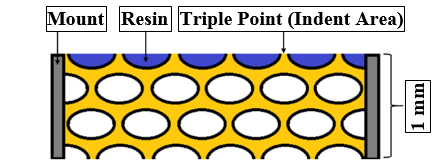
\includegraphics[scale=0.8]{NanoindentSample}
  \captionsetup{justification=centering}
  \caption[Close up of \textit{Hemidactylus} sp.]
   {Schematic of the foam sample for the nanoindentation tests.}
   \label{fig:NanoindentSample}
\end{figure}

\section{Multiscale modelling strategy}
As discussed in introduction, the mechanical behaviour of PU foams depends on the density, the geometric features of the foam and the mechanical behaviour of the solid PU. This section describes the development of a reliable modelling strategy to account for the influence of the density as well as geometrical features of the foam on the mechanical behaviour of PU foams \citep{Chen2015150}. Figure~\ref{fig:Strategy} demonstrates the map for modelling strategy. The first step is to create a realistic geometric model of the foam, including all the geometric features, by means of Laguerre tessellation. To this end, the algorithm for random close packing distribution of spheres is first discussed. Then, the Laguerre tessellation technique is presented. Also, the details of finite element model including finite discretization and material assignment are described. Finally, the validation is performed by comprising simulation results with experimental measurements.
\begin{figure}[hb]
  \centering
  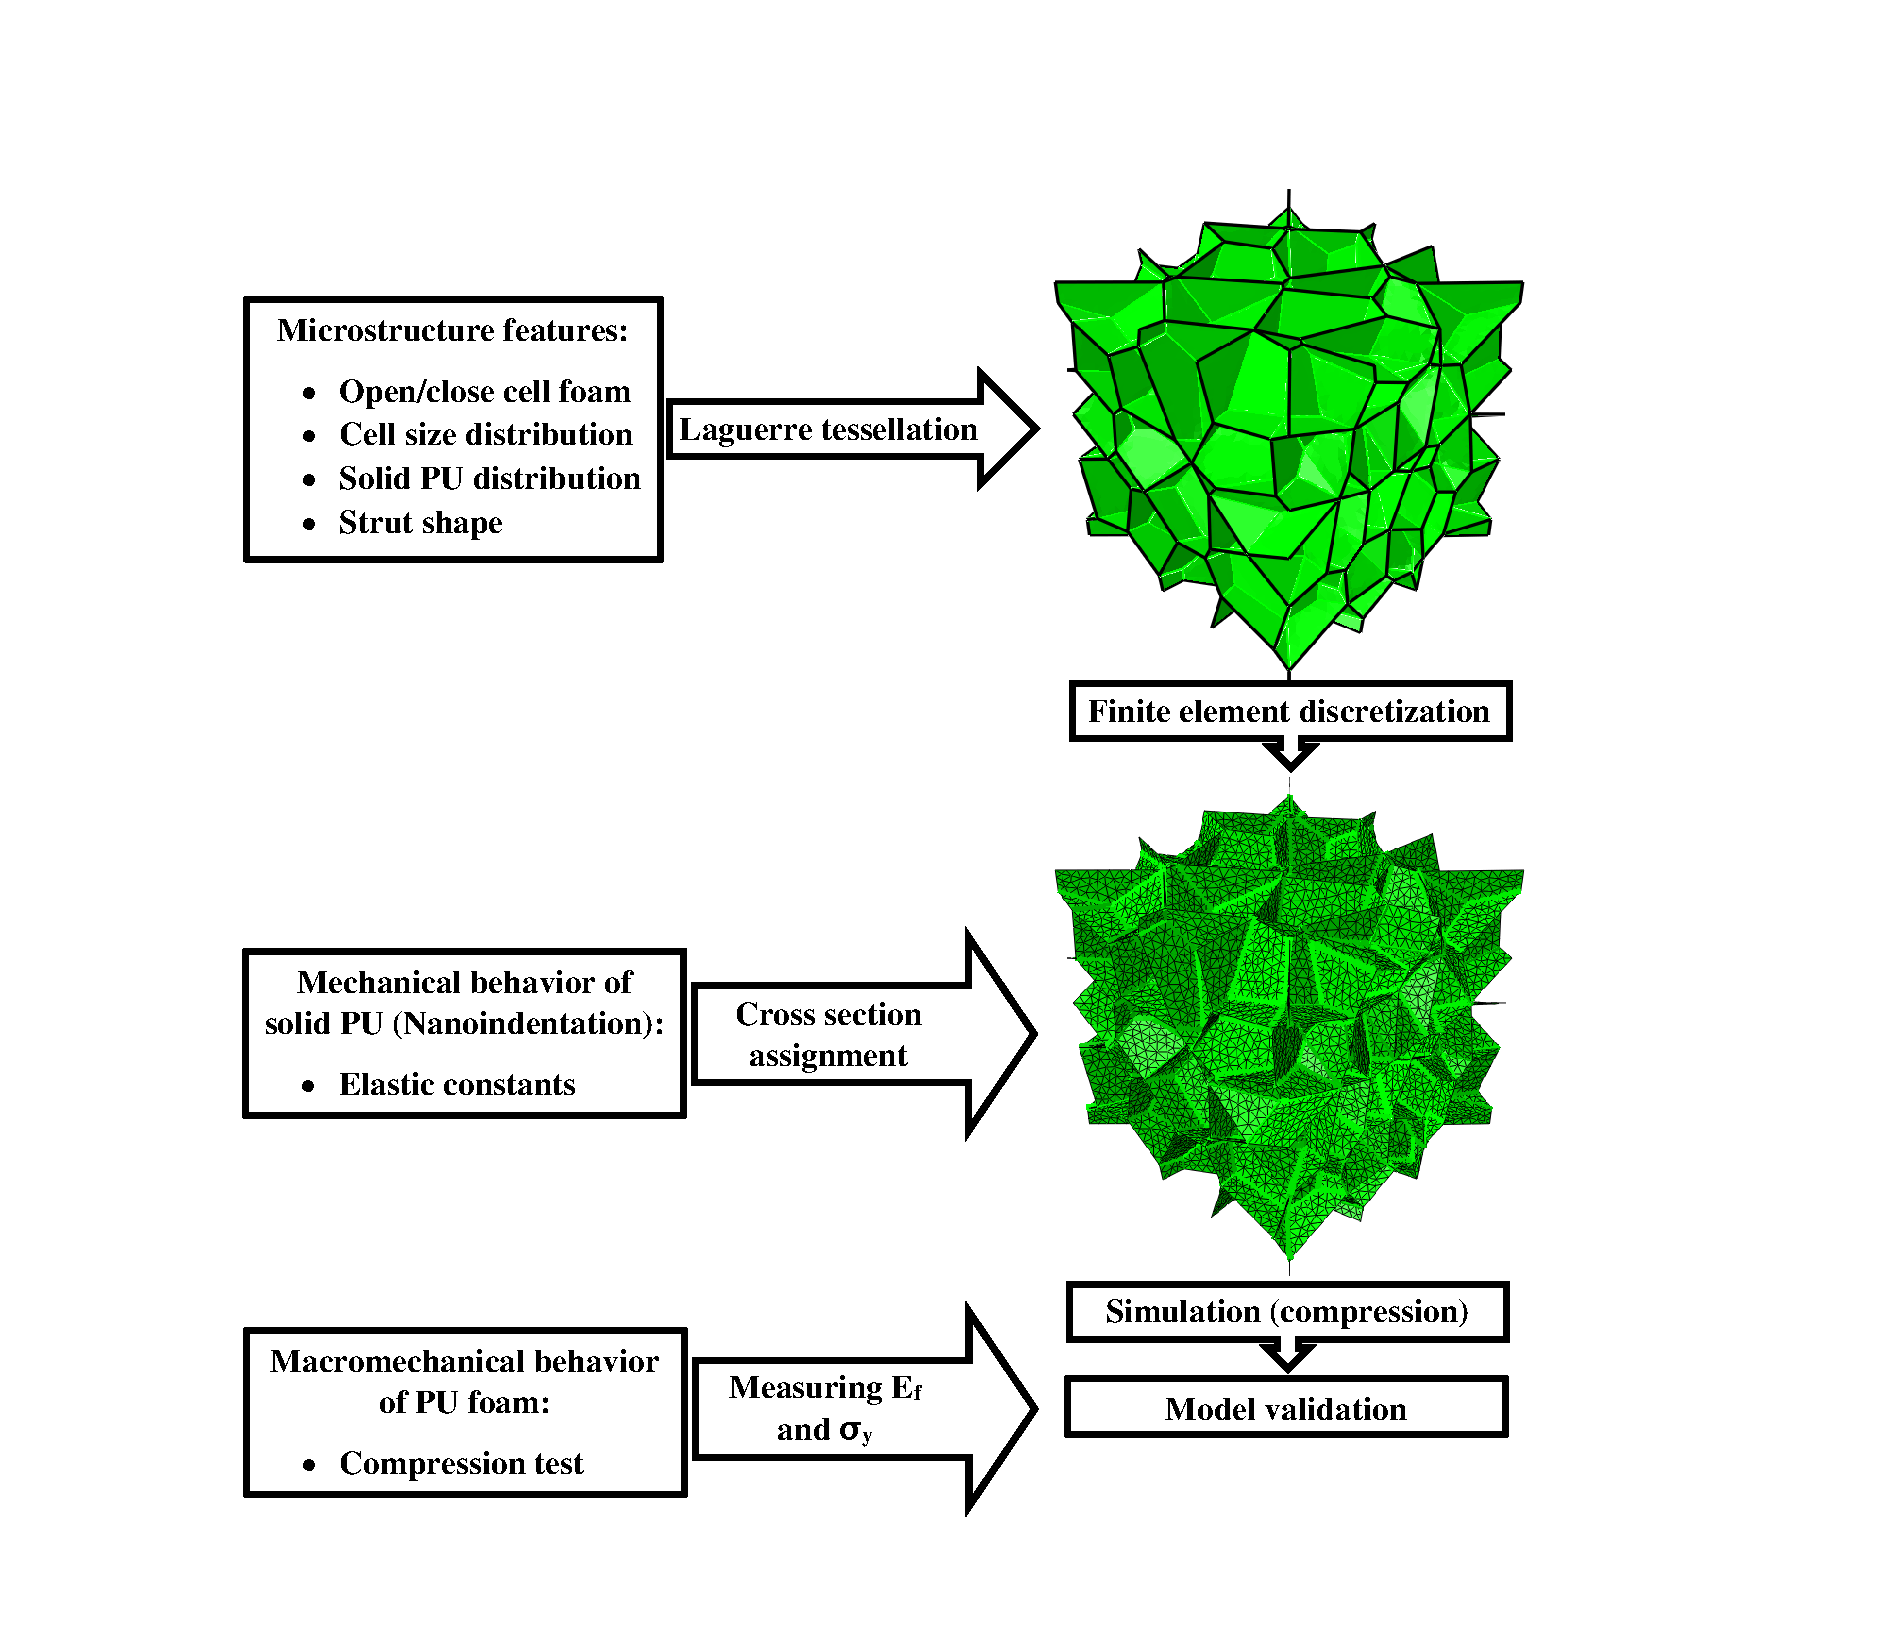
\includegraphics[scale=0.4]{Strategy}
  \captionsetup{justification=centering}
  \caption[Close up of \textit{Hemidactylus} sp.]
   {The strategy map of multiscale modelling.}
   \label{fig:Strategy}
\end{figure}

\subsection{Random packing of spheres}
The foam microstructure is formed by a 3D arrangement of cells. The average cell size is assumed to be the same in all directions and the cell sizes are assume to follow a given statistical distribution characterized by the average cell diameter, $\mu$, and the standard distribution of the cell diameter, $\sigma$. Each cell is assimilated to a sphere with the same diameter and the location of the centers of the cells in the 3D space can be obtained from the positions of the centers of a 3D ensemble of random close packed spheres with the same diameter distribution as the foam.

Dense packing of spheres with higher volume fraction can be achieved using on the collective rearrangement algorithms. Among them, the force biased algorithm is widely used because of its high efficiency \citep{bargiel1991c}.  This algorithm starts with an initial distribution of spheres. In this case, the initial configuration is given by $n_0$ spheres $S($\textit{\textbf{x}}$_i,d_i/2)$  with centers at \textit{\textbf{x}}$_i$  and radii  distributed in a parallelepipedic container. In this step, overlapping of spheres is possible and allowed. Then, the algorithm attempts to reduce the overlaps between spheres using by pushing apart overlapped spheres. After certain number of iterations, repositioning of overlapped spheres is stopped. Then, algorithm attempts to shrink the spheres gradually. This procedure decreases the total amount of overlaps. Once, the total amount of overlaps in new configuration of spheres becomes less than a certain value, the algorithm stops and returns as output the final positions and radii of the spheres. Figure~\ref{fig:PackedSpheres} shows two 3D packed configurations of spheres with volume fraction of 0.6, obtained by force biased algorithm.  The sphere size distribution follows a normal distribution given by the average value $\mu$ and the standard deviation $\sigma$.
\begin{figure}[hb]
  \centering
  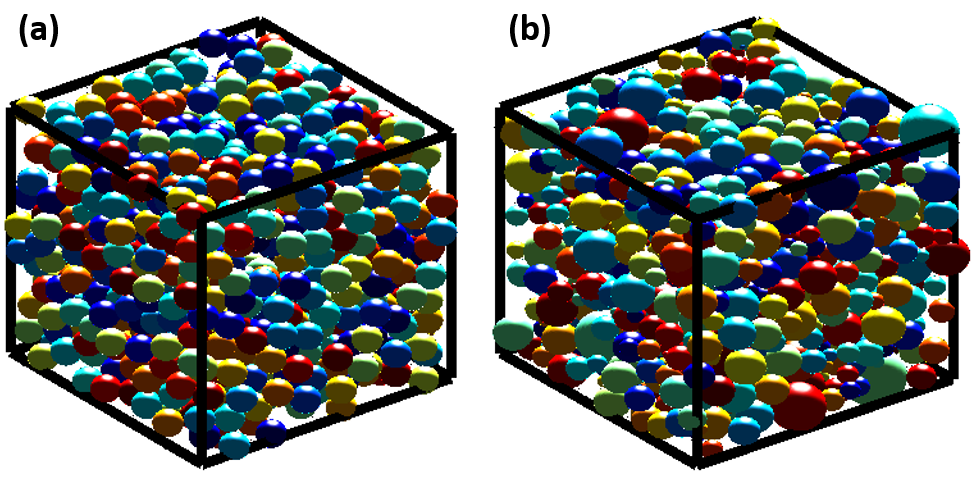
\includegraphics[scale=0.4]{PackedSpheres}
  \captionsetup{justification=centering}
  \caption[Close up of \textit{Hemidactylus} sp.]
   {Two different 3D packed configurations of spheres with volume fraction of 0.6, obtained by force biased algorithm. The sphere size distribution follows a normal distribution given by the average value $\mu$ and the standard deviation $\sigma$. a) $\mu$ = 0.39 and $\sigma$ = 0.01. b) $\mu$ = 0.39 and $\sigma$ = 0.15.}
   \label{fig:PackedSpheres}
\end{figure}

\subsection{Laguerre tessellation}
A tessellation is a locally finite division of D-dimensional space into full dimensional polytopes which intersect only in their boundaries. The most well-known model is the Voronoi tessellation. It is generated by a set $S$ of points in $R^d$ by assigning to the cell of a point $\textit{\textbf{x}}\in S$ all points $\textit{\textbf{y}}\in S$ having $\textit{\textbf{x}}$ as their nearest neighbor in $S$ \citep{Redenbach20091397}. However, in the Voronoi construction cell facets are always equidistant from the generators of their cells. Therefore, the range of cell patterns which can be generated by Voronoi tessellations is limited. This is why weighted generalizations of the Voronoi model are frequently used. One possible generalization is the Laguerre tessellation which is defined as following. 

Let \textbf{\textit{p}}$\ \in R^d$ be a fixed point and $w\ \in R^d$ be a fixed value, called the weight of point \textbf{\textit{p}}. For all \textbf{\textit{x}}$\ \in R^d$, the power of \textbf{\textit{x}} with respect to $($\textbf{\textit{p}}$,w)$ defined as $pow($\textbf{\textit{x}}$,($\textbf{\textit{p}}$,w))$. If $P=\lbrace ($\textbf{\textit{p}}$_1,w_1)$,$($\textbf{\textit{p}}$_2,w_2)$,$\ ...$\ ,$($\textbf{\textit{p}}$_n,w_n)$ $\rbrace$ is a finite set of n weighted points in $R^d$, then, the Laguerre tessellation diagram of $P$ divides $R^d$ into cells, using the power of these points. The cell associated with the $i$-th generator point, $C_i$, is defined by
\begin{equation}
C_i=\lbrace \textbf{\textit{x}}\in R^d:pow(\textbf{\textit{x}},(\textbf{\textit{p}}_i,w_i)) \leq
 pow(\textbf{\textit{x}},(\textbf{\textit{p}}_j,w_j))  \rbrace
\end{equation}

when  all  weights  are  positive,  each  weighted  generator  point $($\textbf{\textit{p}}$,w)\in P$ can  be  interpreted  as  a  sphere 
(denoted $S($\textbf{\textit{p}}$,d/2)$) with radius $d/2=\sqrt[•]{w}\geq0$  centered at point \textbf{\textit{p}}. The power of a point \textbf{\textit{x}} with respect to the 
sphere $S($\textbf{\textit{p}}$,d/2)$ is thus given by $pow($\textbf{\textit{x}},$S($\textbf{\textit{p}}$,d/2)$=$\parallel$ \textbf{\textit{x}}-\textbf{\textit{p}}$\ \parallel^2$-$r^2$. Geometrically, this means that for a point \textbf{\textit{x}} outside the sphere $S($\textbf{\textit{p}}$,d/2)$, the value of $pow($\textbf{\textit{x}},$S($\textbf{\textit{p}}$,d/2))$ is equal to the squared length of the tangent line 
from \textbf{\textit{x}} to $S($\textbf{\textit{p}}$,d/2)$.  The  boundary  between  two  adjacent  cells  generated  by  spheres $S_1=S($\textbf{\textit{p}}$_1,d_1/2)$ and $S_2=S($\textbf{\textit{p}}$_2,d_2/2)$, consists of all points \textbf{\textit{x}}$\ \in R^d$  such that $pow($\textbf{\textit{x}},$S_1)$=$pow($\textbf{\textit{x}},$S_2)$. In other words, the Laguerre 
diagram is the set of the Laguerre cells and forms a space-filling system of convex polytopes (Laguerre 
Voronoi diagram). If $S$ is chosen as a system of non-overlapping spheres, then each cell of Laguerre diagram 
completely contains its generating sphere. Physically, the Laguerre cell of $C_i$ consists of points 
which are closer to seed $P_i$ than other seeds in the Laguerre diagram. As a result of dividing the Euclidean 
space in this manner, the volume distribution of Laguerre cells is almost equal to volume distribution of 
their generating spheres. Because porous materials (e.g. polyurethane foam) are made of cells with specific 
size distribution, their geometry can be constructed by means of Laguerre tessellation. In addition to the 
cell size distribution, Laguerre cells show close averages for both number of faces per each cell and number 
of edges per face, to those found in real PU foams \citep{Fan2004,Rhodes1994}.  

In order to have periodic boundaries in tessellated volume, the geometry created by Laguerre tessellation has to show periodicity in its outer edges and faces. For the sake of simplicity, the strategy to create periodic Laguerre cells is explained in 2D, but the extension to 3D is straightforward. Figure~\ref{fig:Periodic}a represents a packed configuration of circles in a rectangular area of the size $L \times L$, which has been chosen to perform the tessellation. The corresponding Laguerre tessellation is depicted in Figure~\ref{fig:Periodic}b.
\begin{figure}[hb]
  \centering
  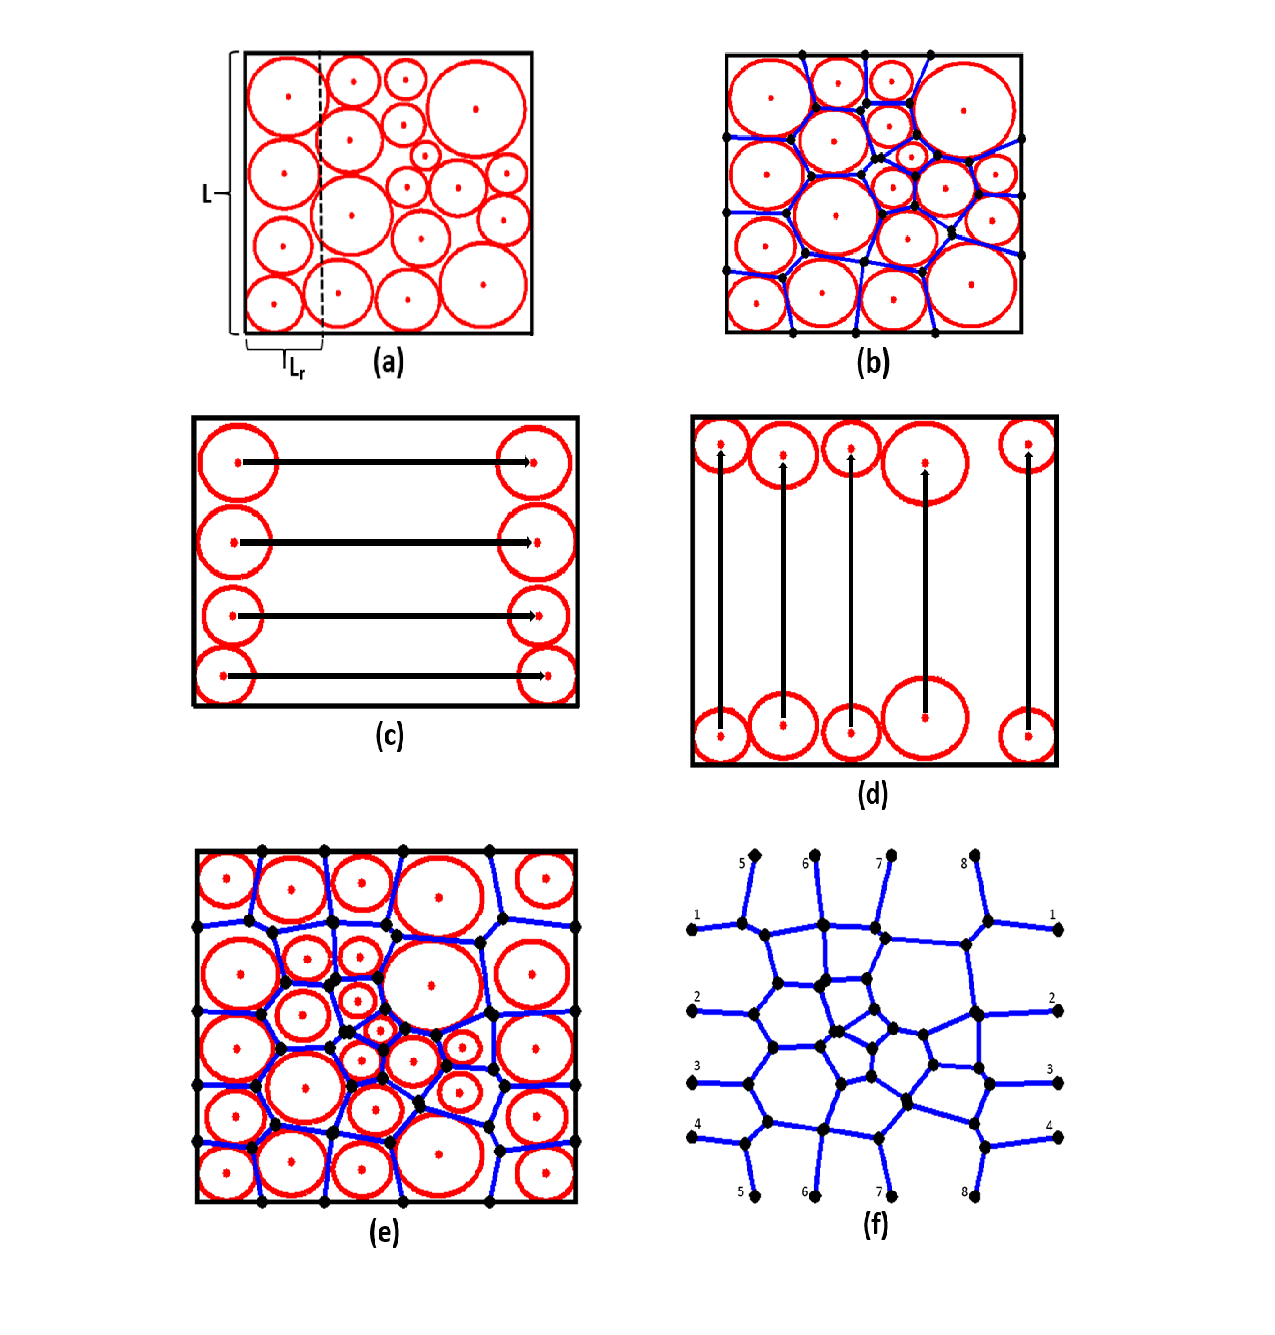
\includegraphics[scale=0.6]{Periodicity}
  \captionsetup{justification=centering}
  \caption[Close up of \textit{Hemidactylus} sp.]
   {a) The initial packed configuration of the circles, b) Image of the edge system of a 2D Laguerre tessellation; Duplication of circles: c) located at the left boundary of the RVE to the right, d) located at the bottom of RVE to the top; e) 2D Laguerre tessellation together with the new circle distribution, f) The new periodic Laguerre tesselation.}
   \label{fig:Periodic}
\end{figure}

The steps to create a periodic geometry are shown in Figure~\ref{fig:Periodic}c to \ref{fig:Periodic}f. The circles located at the left side of the packed configuration of circles are duplicated (i.e. the first column of circles from the left) on the right side and the circles located at the bottom (i.e. the first row of circles form the bottom) are duplicated on the top of the packed configuration of circles, as illustrated by arrows in Figure~\ref{fig:Periodic}c and \ref{fig:Periodic}d, respectively. The new configuration of circles contains more circles and it is used as input for the Laguerre tessellation (Figure~\ref{fig:Periodic}e), which leads to a periodic microstucture, Figure~\ref{fig:Periodic}f. Periodic node-pairs on opposite faces are marked with the same number. Node-pairs 1, 2, 3 and 4 (located on left side of RVE) have the same Y coordinate as their corresponding pairs in opposite side of RVE (right side of the RVE). Similarly, node-pairs 5, 6, 7 and 8 (located on the bottom of RVE) have the same X coordinate as their corresponding pairs in opposite side of the RVE (the top of  the RVE).

It is worth mentioning that a reference distance, $L_r$, has been chosen in order to extract the circles located on the left side of the packed configuration of circles (which should be duplicated later on the right side of the RVE). The choice of $L_r$ depends on the number of circles in RVE and could be adjusted by a trial and error approach. In addition, the cell size distribution is slightly modified by the addition of cells to the primary configuration to achieve the periodicity. These modifications are not expected to modify significantly the elastic and shear moduli, as well as the Poisson’s ratio of the polymeric foam \citep{Köll201611}.  

The same methodology can be used to achieve the periodicity in 3D and an example corresponding to a periodic cubic RVE with 100 cells with a normal volume distribution given by $\mu$ = 0.39 and $\sigma$ = 0.15 is depicted in Figure~\ref{fig:Periodic100Cell}.   
\begin{figure}[hb]
  \centering
  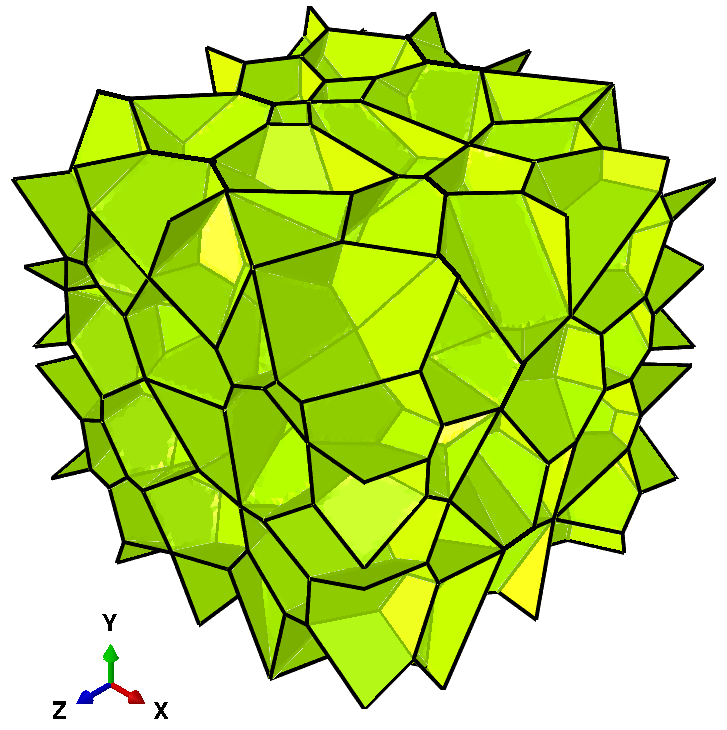
\includegraphics[scale=.6]{Periodic100Cell}
  \captionsetup{justification=centering}
  \caption[Close up of \textit{Hemidactylus} sp.]
   {Periodic Laguerre tessellation of a cubic RVE containing 100 cells.}
   \label{fig:Periodic100Cell}
\end{figure}
\subsection{Finite element model}
The periodic cubic unit cell of dimensions $L \times L \times L$ was generated using Laguerre tessellation technique as a representative volume element (RVE) of the foam microstructure (Figure~\ref{fig:Periodic100Cell}). The tessellated volume was exported to the open-source software Gmsh \citep{Gmsh} to perform the finite element discretization.

As mentioned in the introduction, solid PU can be located in faces or edges (struts) of cells in the PU foam microstructure. In the current study, Euler-Bernoulli beam elements type B31 and shell elements type S3R are used to represent struts and faces, respectively. If $V_{RVE}$ and $\rho_f$ are the volume of the RVE and the density of the foam, the total mass of solid PU in the RVE, $m_{PU}$ is given by,
\begin{equation}
m_{PU}=V_{RVE}\ \rho_f
\end{equation}
and the total volume of solid PU in the RVE ($V_{PU}$) is
\begin{equation}
V_{PU}=\frac{m_{PU}}{\rho_{PU}}
\end{equation}
where $m_{PU}$ is the mass of the solid PU and   $\rho_{PU}$ the density of the solid PU, 1200 $Kg/m^3$ \citep{Mills2007xvii}. $V_{PU}$ should be assigned to both faces and struts so that the final configuration of RVE represents the real foam microstructure. If the volume fraction of solid PU in the faces is $V_{faces}$, the remaining solid PU goes to the struts ($V_{struts}$). Assuming the same thickness for all faces in the foam microstructure, the thickness of the shell elements is given by,
\begin{equation}
t_{ShellElements}=\frac{V_{faces}V_{PU}}{Total \ area \ of \ faces \in RVE}
\label{ThicknessShellElement}
\end{equation}
Moreover, experimental measurements revealed that the amount of material in the struts is approximately proportional to the strut length (Figure~\ref{fig:StrutContent}). Thus, if the total length of the struts in the RVE is $L_t$, the volume $V_i$ corresponding to the strut $i$ of length of $L_i$ is 
\begin{equation}
V_i=\frac{V_{struts}V_{PU}}{L_t}L_i
\label{TotalLenStruts}
\end{equation}
\begin{figure}[hb]
  \centering
  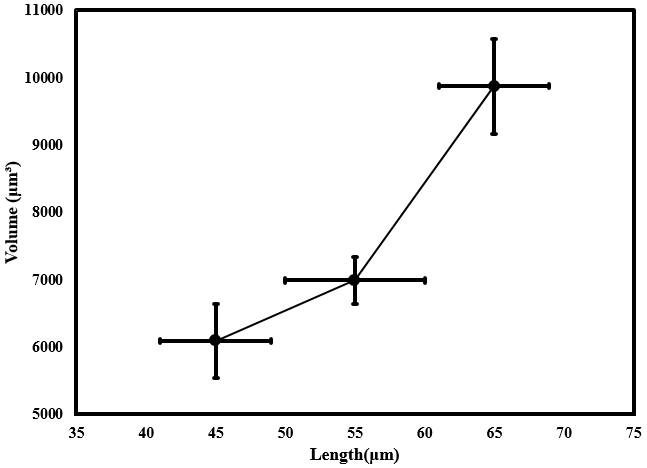
\includegraphics[scale=0.6]{StrutContent}
  \captionsetup{justification=centering}
  \caption[Close up of \textit{Hemidactylus} sp.]
   {Average volume content of struts as a function of average length.}
   \label{fig:StrutContent}
\end{figure}
In addition, the variation of the strut cross-section along the length was obtained by X-ray computed microtomography is shown in Figure~\ref{fig:StrutCrossSection} and can be expressed as
\begin{equation}
A(e)=A_0f(e)=A_0(2.77e^4+0.962e^3+3.403e^2-0.229e+1.025)
\end{equation} 
where $A_o$ is the area of the cross section at the midspan of the strut.

In order to reduce the computational cost, more number of beam elements were used to mesh the long struts, and fewer elements were used to mesh the shorter ones. Therefore, the cross sectional area variation along the strut was described by assigning different cross sectional area to each beam element in the strut depending on the number of assigned elements to each strut. If $N$ is the number of elements in the strut $i$ with volume content of $V_i$, and $a_1$,$a_2$,$...$,$a_N$ are the normalized cross sectional areas of these $N$ beam elements, the normalized cross sectional area for each beam element can be obtained by,
\begin{equation}
a_1=\int_{-0.5}^{b-0.5}f(e)de, a_2=\int_{b-0.5}^{(2b)-0.5}f(e)de, ..., a_N=\int_{((N-1)b)-0.5}^{(Nb)-0.5}f(e)de 
\end{equation}
where $b=1/N$. If the length of the beam elements is $B$, the cross sectional areas of these $N$ beam elements ($A_1, A_2, ..., A_N$) are given by,
\begin{equation}
A_1=\frac{\vert a_1 \vert V_i}{B \sum_{i=1}^{N}\vert a_i \vert}, A_2=\frac{\vert a_2 \vert V_i}{B \sum_{i=1}^{N}\vert a_i \vert}, ..., A_N=\frac{\vert a_N \vert V_i}{B \sum_{i=1}^{N}\vert a_i \vert}
\end{equation}
$A_1, A_2, ..., A_N$ are calculated for each set of  beam elements in each strut and are  assigned to  the beam elements. It should be mentioned that the trapezoidal beam section was employed as the cross section of beam elements since its shape is close enough to the three-cusp hypocycloid cross-section of struts in the foam microstructure \citep{Jang20081845}. 

Faces are discretized with S3R shell elements of constant thickness. It should be noted that shell elements and beam elements share the nodes on the struts. As a result, the number of shell elements in the RVE is controlled by the number of beam elements in the struts. Thus, increasing the number of beam elements in the struts provides a more accurate description of cross sectional variation along the struts, but leads to a large increase in number of shell elements. The discretization of a RVE with 100 cells and 149730 elements 
is shown in Figure~\ref{fig:Discretized}. The inset shows clearly the cross sectional area variation along the struts.
\begin{figure}[hb]
  \centering
  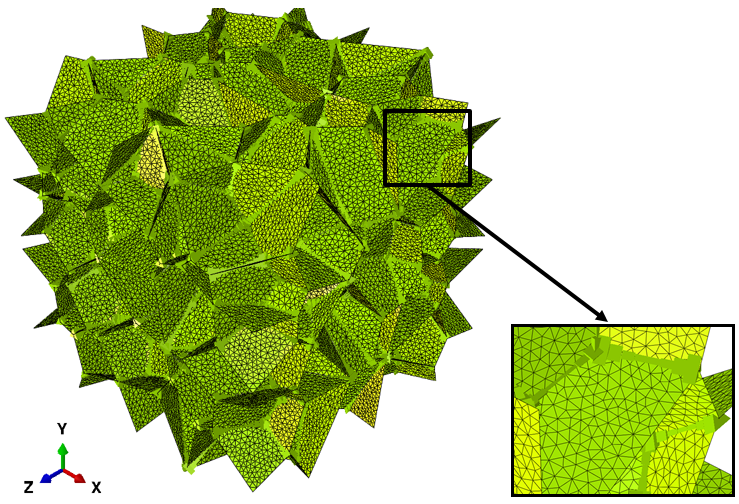
\includegraphics[scale=0.6]{Discretized}
  \captionsetup{justification=centering}
  \caption[Close up of \textit{Hemidactylus} sp.]
   {Finite element discretization of a periodic RVE with 100 cells.}
   \label{fig:Discretized}
\end{figure}

In current study, periodic boundary conditions are used to perform the compressive deformation \citep{HUET1990813,Segurado20022107}. If $X$, $Y$ and $Z$ stand for the Cartesian coordinates, the periodic boundary conditions could be expressed in terms of three displacement vectors \textbf{\textit{u}}$_X$, \textbf{\textit{u}}$_Y$ and \textbf{\textit{u}}$_Z$ relating the relative displacement of a set of master nodes (M0, MX, MY and MZ which are located in positions of $(0,0,0)$, $(L,0,0)$, $(0,L,0)$ and $(0,0,L)$, respectively) laying in opposite faces of the cubic RVE (Figure~\ref{fig:PBC}). Therefore, \textbf{\textit{u}}$_X$=\textbf{\textit{u}}$^\mathrm{MX}$-\textbf{\textit{u}}$^\mathrm{M0}$, \textbf{\textit{u}}$_Y$=\textbf{\textit{u}}$^\mathrm{MY}$-\textbf{\textit{u}}$^\mathrm{M0}$ and \textbf{\textit{u}}$_Z$=\textbf{\textit{u}}$^\mathrm{MZ}$-\textbf{\textit{u}}$^\mathrm{M0}$. Mathematically, the periodic boundary condition can be expressed as following equations
\begin{equation}
\textbf{\textit{u}}(L,y,z)-\textbf{\textit{u}}(0,y,z)=\textbf{\textit{u}}^\mathrm{MX}-\textbf{\textit{u}}^\mathrm{M0}=\textbf{\textit{u}}_X
\label{9}
\end{equation}
\begin{equation}
\textbf{\textit{u}}(x,L,z)-\textbf{\textit{u}}(x,0,z)=\textbf{\textit{u}}^\mathrm{MY}-\textbf{\textit{u}}^\mathrm{M0}=\textbf{\textit{u}}_Y
\label{10}
\end{equation}
\begin{equation}
\textbf{\textit{u}}(x,y,L)-\textbf{\textit{u}}(x,y,0)=\textbf{\textit{u}}^\mathrm{MZ}-\textbf{\textit{u}}^\mathrm{M0}=\textbf{\textit{u}}_Z
\label{11}
\end{equation}
while, $\textbf{\textit{u}}(L,y,z)-\textbf{\textit{u}}(0,y,z)$ in equation \ref{9} expresses the relative displacement for each pair of nodes like 
i and  i$^\prime$ located on RVE surfaces $x=0$ and $x=L$, respectively. Similarly, $\textbf{\textit{u}}(x,L,z)-\textbf{\textit{u}}(x,0,z)$ in equation \ref{10} expressed the relative displacement for each pair of nodes like j and j$^\prime$ located on the RVE surfaces at $y=0$ and $y=L$, respectively , and finally, $\textbf{\textit{u}}(x,y,L)-\textbf{\textit{u}}(x,y,0)$ in equation \ref{11} is the relative displacement 
for each pair of nodes like k and k$^\prime$  located on the RVE surfaces $z=0$ and $z=L$, respectively.  In other words, 
the relative displacement of a pair of nodes lying on opposite faces is equal to the displacement between 
the corresponding pair of master nodes. The different loading states (e.g. compression) could be introduced 
imposing displacement to these master nodes. Each master node contains the reaction force generated by 
all the nodes lying on its corresponding surface. For instance, a uniaxial compressive strain ($\delta<0$) along 
the X axis is introduced by setting $\textbf{\textit{u}}^\mathrm{M0}=(0,0,0)$, $\textbf{\textit{u}}^\mathrm{MX}=(\delta,0,0)$, $\textbf{\textit{u}}^\mathrm{MY}=(0,\textbf{\textit{u}}_Y,0)$ and $\textbf{\textit{u}}^\mathrm{MZ}=(0,0,\textbf{\textit{u}}_Z)$, 
where $\textbf{\textit{u}}_Y$, and $\textbf{\textit{u}}_Z$ are obtained from the conditions: 
\begin{equation}
\int_{\Omega_Y}t_Yd\Omega \ \ \ \ \ \Omega_Y:y=L
\end{equation}
\begin{equation}
\int_{\Omega_Z}t_Zd\Omega \ \ \ \ \ \Omega_Z:z=L
\end{equation}

Periodic boundary conditions can be introduced in the model using the equation command in ABAQUS 
(*EQUATION).  In  this  case, for  each  pair  of  nodes,  6  equations,  corresponding to  the  all  6  degrees  of 
freedom in nodes, are needed. 
\begin{figure}[hb]
  \centering
  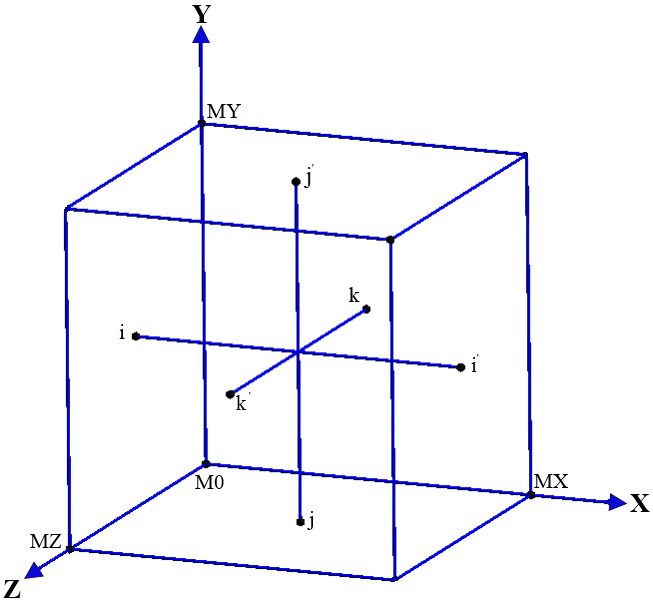
\includegraphics[scale=0.6]{PBC}
  \captionsetup{justification=centering}
  \caption[Close up of \textit{Hemidactylus} sp.]
   {Schematic of the RVE with length $L$ together with its master nodes in 3D.}
   \label{fig:PBC}
\end{figure} 
The finite element analysis is performed using Abaqus/Standard and the material was assumed to follow elastic, isotropic solid. The elastic and shear moduli of the solid PU were obtained by instrumented nanoindentation ($E_{PU}=2.4 \ \mathrm{GPa}$, $G_{PU}=0.9 \ \mathrm{GPa}$) and the Poisson's ratio $\nu=0.35$ was obtained from the literature \citep{Mills2007xvii}. The RVE size and the discretization were analyzed to ensure that the results were independent from both factors. 

\section{Experimental results}

\subsection{Microstructure of PU foam}

The microstructure of the PU foam 1-3CPW30.2 is shown in the SEM micrographs in Figure~\ref{fig:SEMmicrostructure}. The sample is made up of closed-cells. The average diameter of the cells and the aspect ratio parallel and perpendicular to the rising direction was measured from 10 micrographs, including approximately 250 cells. The average diameter of  250$\pm$32 and 255$\pm$50 were obtained in parallel and perpendicular to the rising direction, respectively. Moreover, the aspect ratio parallel and perpendicular to the rising direction were 1.30$\pm$0.09 and 1.30$\pm$0.14, respectively.    
 
The cell aspect ratio of specimen 1-3CPW30.2 in both directions of parallel and perpendicular to rising direction of foam were small ($\approx$ 1.3) and very similar and this confirms the isotropic morphology of this foam. Moreover, the average thickness of the faces, measured by scanning electron microscopy, was 0.40$\pm$0.25 \SI{}{\micro\metre} Figure~\ref{fig:FaceThickness}.

\begin{figure}[hb]
  \centering
  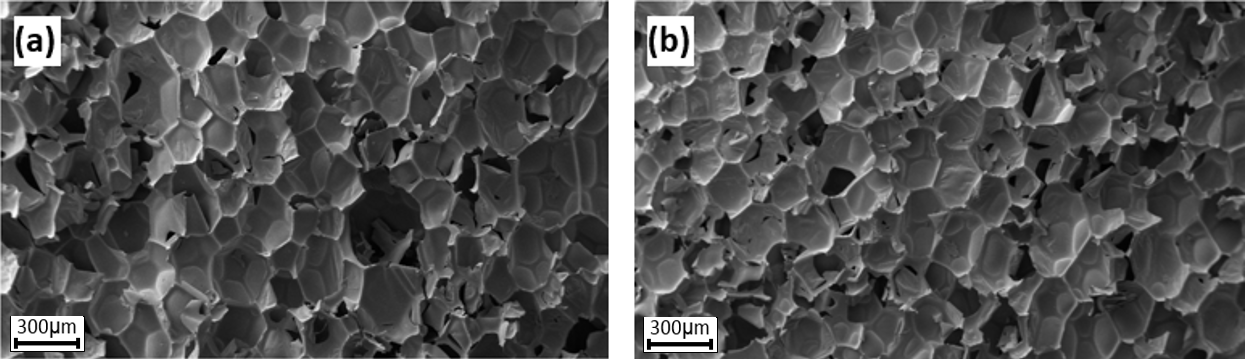
\includegraphics[scale=0.3]{SEMmicrostructure}
  \captionsetup{justification=centering}
  \caption[Close up of \textit{Hemidactylus} sp. ]
   {SEM micrographs: (a) parallel and (b) perpendicular to rising direction of the 1-3CPW30.2.}
   \label{fig:SEMmicrostructure}
\end{figure}

\begin{figure}[hb]
  \centering
  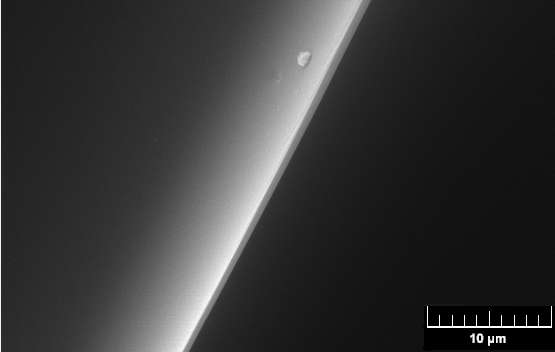
\includegraphics[scale=0.6]{FaceThickness}
  \captionsetup{justification=centering}
  \caption[Close up of \textit{Hemidactylus} sp. ]
   {Scanning electron micrograph of the cross-section of a face in the PU foam.}
   \label{fig:FaceThickness}
\end{figure}

The cell size distribution of the 1-3CPW30.2 foam was studied using X-ray computed microtomography, which followed a normal distribution with mean value $\mu=$  0.39 and standard deviation $\sigma=$ 0.15 (Figure~\ref{fig:CellSizeDist}). The strut shape was determined by means of XCT for 1-3CPW30.2, Figure~\ref{fig:StrutShape}. Measurements were conducted in several different regions of the foam and ten struts were measured in each region. The cross-sectional area of each slice of strut, normalized by the value at the mid-span, $A_0$, is plotted against the normalized length for several struts in Figure~\ref{fig:StrutCrossSection}. Different polynomial functions were used to fit the experimental data and the best agreement was reached with the following function: 
\begin{equation}
A(e)=A_0f(e)=A_0(2.770e^4+0.962e^3+3.403e^2-0.229e+1.025)
\end{equation}
\noindent where $e=l/l_0$ is the position along the strut of  length $l$\cite{Jang20081845}.

\begin{figure}[hb]
  \centering
  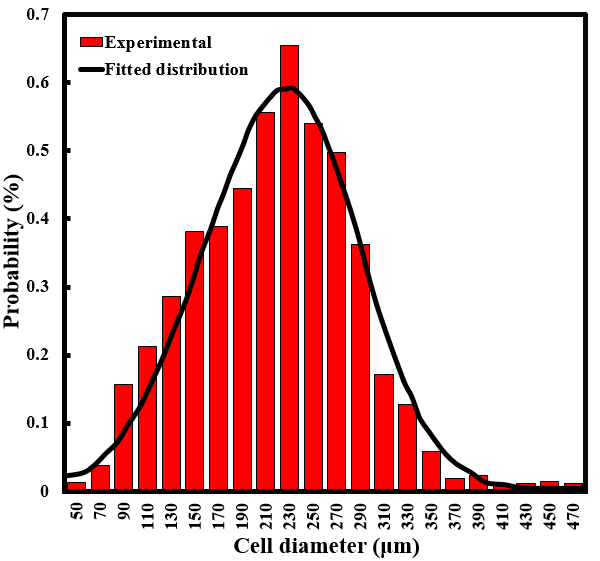
\includegraphics[scale=0.8]{CellSizeDist}
  \captionsetup{justification=centering}
  \caption[Close up of \textit{Hemidactylus} sp. ]
   {The measured cell size distribution together with fitted distribution.}
   \label{fig:CellSizeDist}
\end{figure}

\begin{figure}[hb]
  \centering
  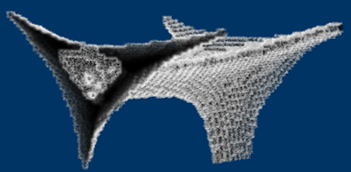
\includegraphics[scale=1]{StrutShape}
  \captionsetup{justification=centering}
  \caption[Close up of \textit{Hemidactylus} sp. ]
   {XCT volume of a strut.}
   \label{fig:StrutShape}
\end{figure}

\begin{figure}[hb]
  \centering
  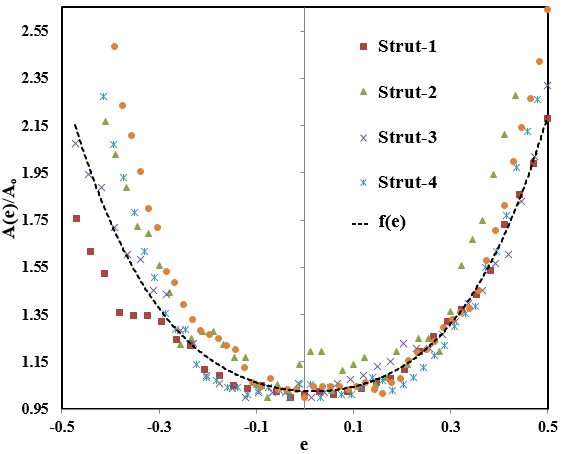
\includegraphics[scale=0.8]{StrutCrossSection}
  \captionsetup{justification=centering}
  \caption[Close up of \textit{Hemidactylus} sp. ]
   {The strut cross-section area variation.}
  \label{fig:StrutCrossSection}
\end{figure}

\subsection{Elastic properties of the solid PU}
Oyen establishes a simple experimental technique for the analysis of time-dependent mechanical behavior of materials using load-controlled spherical indentation \cite{oyen2005}. Elastic-viscoelastic correspondence analysis has been used to generate solutions for indentation creep at fixed load following loading to peak at constant rates over experimentally reasonable time frames. Figure~\ref{fig:SchematicLoadUnload}, shows the loading protocol that has been used as a ramp-and-hold creep test.  
\begin{figure}[hb]
  \centering
  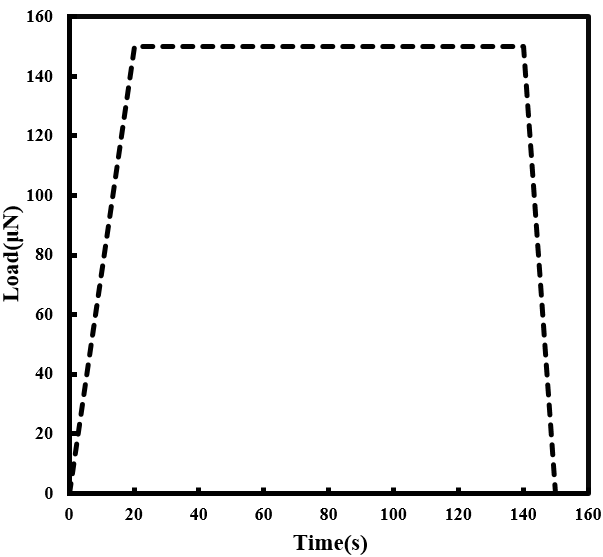
\includegraphics[scale=0.6]{SchematicLoadUnload}
  \captionsetup{justification=centering}
  \caption[Close up of \textit{Hemidactylus} sp. ]
   {Ramp-and-hold loading-time protocol.}
  \label{fig:SchematicLoadUnload}
\end{figure}

The indentation depth $h$ can be expressed as a function of the indentation load $P$ in the elastic regime for a spherical indenter according to \citep{1960JAM....27..438L}
\begin{equation}
h^{3/2}=\frac{3}{4\ \sqrt[•]{R}}P\frac{1-\nu^2}{E}
\end{equation}
where $R$ is the tip radius of the spherical indenter. For an incompressible material ($\nu=0.5$), Eq. (2) can be written as 
\begin{equation}
h^{3/2}=\frac{3}{8\ \sqrt[•]{R}}[\frac{P}{2G}]
\end{equation}
where $G$ is the shear modulus. Replacing the term $\displaystyle{\frac{P}{2G}}$  with the viscoelastic Boltzmann integral equation (\citep{1960JAM....27..438L}) leads to
\begin{equation}
h^{3/2}=\frac{3}{8\ \sqrt[•]{R}}\int\limits_0^tJ(t-u)\frac{dP}{du}du
\end{equation}
where $J(t)$ is the material creep function defined as the strain, $\varepsilon(t)$ , divided by the maximum stress \citep{Desprat20052224}. In addition, $u$ is a dummy variable which is used to solve the integral. It should be noted that there are many forms of material creep functions which they come from different material models. They can be used to describe the creep behavior of different material types. In this study, standard linear viscoelastic solid model used that gives delayed elasticity and allows to obtain an instantaneous elastic modulus (see Eq.\eqref{eq:4.7}). The above integral should be solved separately for the loading and holding time, therefore the loading conditions can be written 
\begin{eqnarray}
P(t) =kt,&0\leq t \leq t_R  \nonumber \\
\\
P(t) =P,&t_R\leq t \nonumber 
\end{eqnarray}
where $t_R$ is the time corresponding to the end of loading. Thus,
\begin{eqnarray}
\label{eq:4.6}
h^{3/2}(t)=\frac{3}{8\ \sqrt[•]{R}}\int\limits_0^tJ(t-u)kdu,&0\leq t \leq t_R  \nonumber \\
\\
h^{3/2}(t)=\frac{3}{8\ \sqrt[•]{R}}\int\limits_{t_R}^tJ(t-u)kdu,&t_R\leq t \nonumber 
\end{eqnarray}
The solutions to these integral equations depend on material creep function $J(t)$. In this study, $J(t)$ has the form 
\begin{equation}
J(t)=C_0-C_1exp\left(\frac{-t}{\tau_1}\right)-C_2exp\left(\frac{-t}{\tau_2}\right)
\label{eq:4.7}
\end{equation}
\begin{figure}[hb]
  \centering
  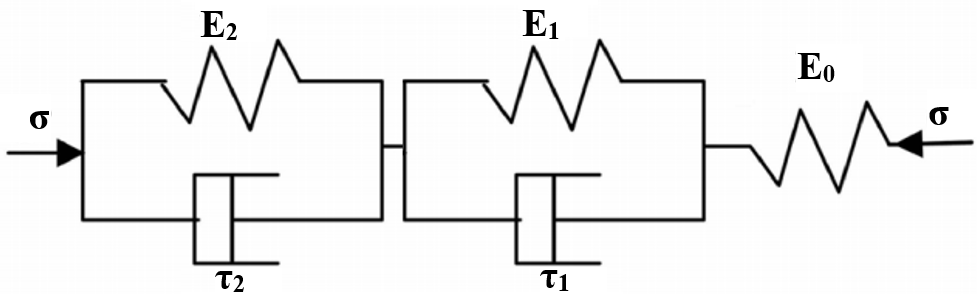
\includegraphics[scale=0.4]{ViscoelasticModel}
  \captionsetup{justification=centering}
  \caption[Close up of \textit{Hemidactylus} sp. ]
   {Standard linear viscoelastic solid model including one elastic spring in series with two Kelvin parallel spring and dashpot elements.}
  \label{fig:ViscoelasticModel}
\end{figure}
which corresponds to a standard linear viscoelastic solid model (one spring in series with two Kelvin parallel spring and dashpot elements), Figure~\ref{fig:ViscoelasticModel}. stand for the elastic modulus of the spring components;  are viscosities of the dashpot components and  is applied stress.

The solution of Eq.\eqref{eq:4.6} for the creep function given by Eq.\eqref{eq:4.7} leads to
\begin{equation}
h^{3/2}(t)=\frac{3k}{8\ \sqrt[•]{R}}\left\{C_0t_R-\sum_{i=1}^{2} C_i\tau_i exp\left(\frac{-t}{\tau_i}\right) \left[exp\left(\frac{t_R}{\tau_i}\right)-1\right]\right\},t_R\leq t
\label{eq:4.8}
\end{equation}
The creep function, Eq.\eqref{eq:4.7}, can be related quantitatively to the shear creep function $G(t)$ \citep{johnson1985contacMech}, 
\begin{equation}
G(t)=\frac{1}{J(t)}
\label{eq:4.9}
\end{equation}
and the instantaneous shear modulus can be calculated in this particular case as \citep{oyen2005}
\begin{equation}
G=\frac{1}{2(C_0-(C_1+C_2))}
\label{eq:4.10}
\end{equation}
while the instantaneous elastic modulus is given by \citep{johnson1985contacMech}
\begin{equation}
E=2G(1+\nu)
\label{eq:4.11}
\end{equation}
Eq.\eqref{eq:4.7} was fitted to the experimental data obtained from the spherical nanodindention of the solid PU vertices within the foam to obtain the viscoelastic properties of the material. To this end, the experimental load-displacement curves had to be corrected to remove the extra compliance induced by the presence of the resin in the pores of the foam. Nanoindentation tests were also performed on both infiltrated resin within the foam pores and on the bulk resin specimen. The load-displacement curves obtained by performing nanoindentation on infiltrated resin inside the foam pores were corrected by the same amount of compliance and then these corrected curves were used to calculate the elastic modulus of the infiltrated resin. Subsequent comparison between the measured elastic modulus for resin inside the pores and the elastic modulus for the bulk resin demonstrated the good agreement between the two measured values validating the applied compliance. Accordingly, the same compliance value used to correct the load-displacement curves of PU solid material. Figure~\ref{fig:LoadDispNano} shows the original and corrected load-displacement curves. It is clear that after correction, the whole curve has been shifted to the left. It means that the extra displacement which was the result of the deformation of the supporting microstructure during loading has been removed. This shift to the left caused by the reduction on the displacement has been shown by an arrow in Figure~\ref{fig:LoadDispNano}.
\begin{figure}[hb]
  \centering
  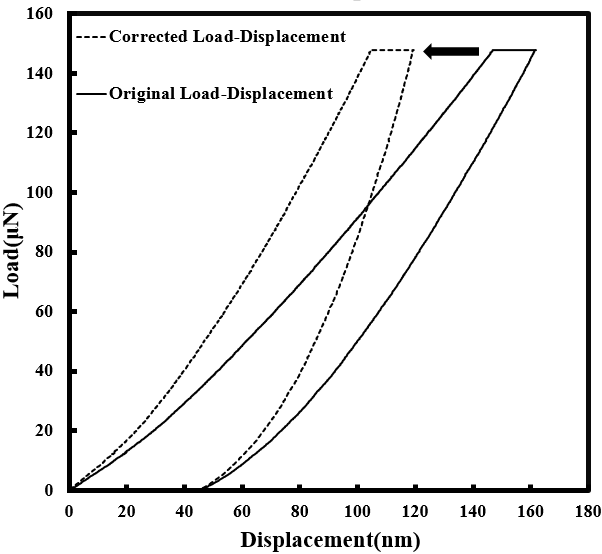
\includegraphics[scale=0.7]{LoadDispNano}
  \captionsetup{justification=centering}
  \caption[Close up of \textit{Hemidactylus} sp. ]
   {Original and corrected load-displacement curves of 1-3CPW30.2.}
  \label{fig:LoadDispNano}
\end{figure}

An example of displacement-time curves for PU foam samples is shown in Figure~\ref{fig:TimeDispNano}. Indentation creep tests were performed at 150 \SI{}{\micro\N} with a 20 s loading time followed by a holding time of 120 s and unloading in 10 s.  The creep deformation data were fit to Eq.\eqref{eq:4.7} and the values of time constants ($\tau_1$ and $\tau_2$) and amplitude coefficients ($C_0$, $C_1$ and $C_2$) were computed by the least squares method. Then, $G$ and $E$ were calculated using Eq.\ref{eq:4.10} and Eq.\ref{eq:4.11}, respectively. Summary of results for elastic moduli of specimens 1-3CPW30.2 is shown in Table 2. It also should be noted that the Poisson’s ratio of PU solid material  was chosen as 0.35 \cite{oyen2005}.
\begin{figure}[hb]
  \centering
  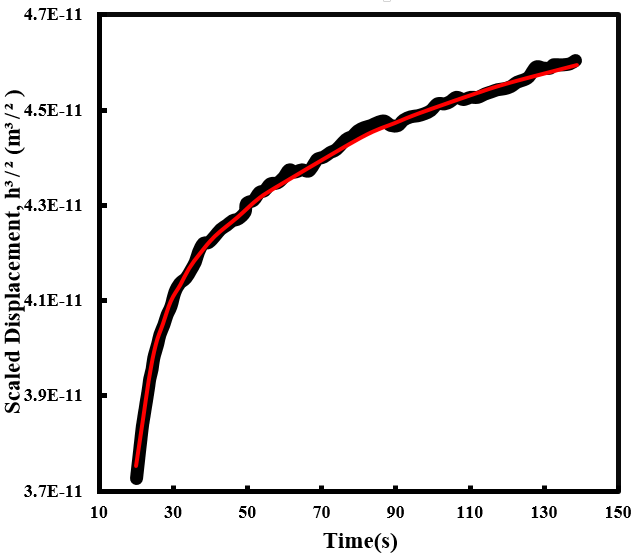
\includegraphics[scale=0.5]{TimeDispNano}
  \captionsetup{justification=centering}
  \caption[Close up of \textit{Hemidactylus} sp. ]
   {Indentation depth–time curve for PU solid material 1-3CPW30.2. The solid red line corresponds to Eq.\eqref{eq:4.7} fitted to experimental curve between 20s and 140s.}
  \label{fig:TimeDispNano}
\end{figure}

\begin{center}
Table 2: Amplitude coefficients and mechanical properties of the solid PU materials
\end{center}
\begin{center}
\begin{tabular}{cccccc}
\hline 
Sample & Amplitude coefficients($\displaystyle{\mathrm{\frac{1}{MPa}}}$) &  Mechanical properties($\mathrm{GPa}$) & • \\ 
\hline 
• & \ \ $C_1$ \ \ \ \ \ \ \ \ \ $C_2$ \ \ \ \ \ \ \ \ \ $C_3$ \ \ &$G$ \ \ \ \ \ \ \ \ \ \ \ \ \ \ \ \ \ \ $E$ \\ 
\hline 
1-3CPW30.2 &1.02e-09 \ 1.25e-10 \ 1.18e-10 & \ \ 0.9$\pm0.03$ \ \ \ \ \ \ \ \ \ 2.40$\pm$0.10 \\ 
\hline 
\end{tabular} 
\end{center}

The AFM (atomic force microscope) micrograph of indented area (i.e. vertex) after unloading is shown in Figure~\ref{fig:AFM}. There was no trace of indentation after unloading and this indicates that the material was in the viscoelastic regime, according to the assumptions in the model. 
\begin{figure}[hb]
  \centering
  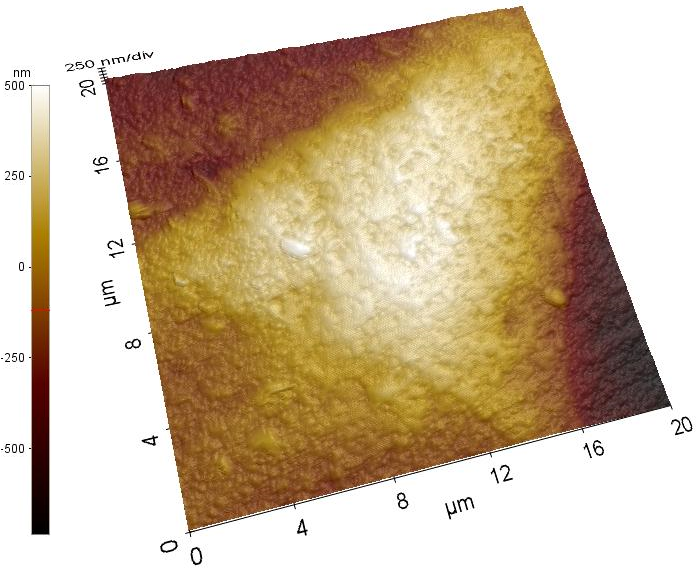
\includegraphics[scale=0.5]{AFM}
  \captionsetup{justification=centering}
  \caption[Close up of \textit{Hemidactylus} sp. ]
   {AFM photograph taken from vertex after unloading.}
  \label{fig:AFM}
\end{figure}

\subsection{Compression result of PU foam}
The representative engineering stress-engineering strain curve of the 1-3CPW- 30.2 foam tested in compression at ambient temperature are plotted in Figure~\ref{fig:StressStrainCurve}. It stand for the mechanical behavior in compression parallel and perpendicular to the rising direction. They show a clear isotropy in the elastic modulus and the yield strength which is in good agreement with the microstructural isotropy of the foam. In addition, the foam loaded in either parallel or perpendicular to the rising direction showed a load drop after the yield point. This drop seems to indicate that the load drop was induced by the sudden collapse by buckling of the struts and faces after yielding. This phenomenon is more discussed in modelling results section.
\begin{figure}[hb]
  \centering
  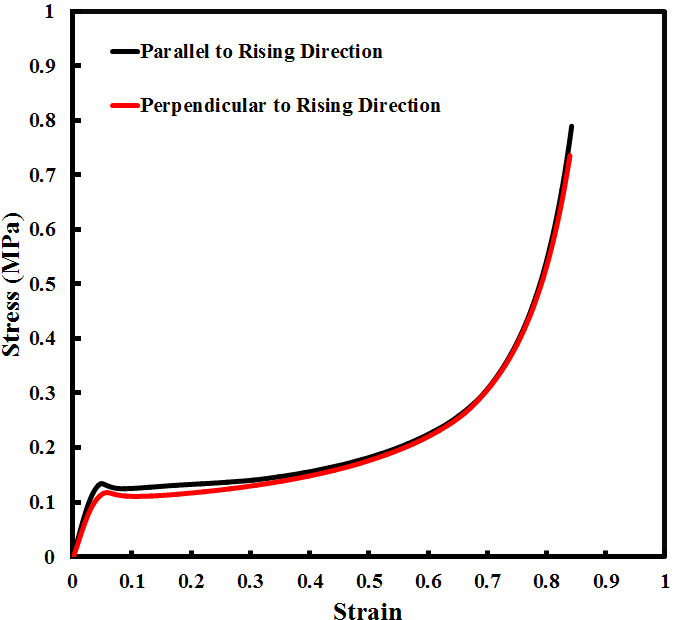
\includegraphics[scale=0.6]{StressStrainCurve}
  \captionsetup{justification=centering}
  \caption[Close up of \textit{Hemidactylus} sp. ]
   {Compressive engineering stress-engineering strain curve of 1-3CPW30.2 at room temperature.}
  \label{fig:StressStrainCurve}
\end{figure}


\section{Modelling results}
In order to build up our model as well as for the model validation, the rigid PU foam 1-3CPW30.2 described in section 2 was chosen as a case study. 

\subsection{RVE and mesh size sensitivity}
The size of the RVE (i.e. number of cells in the RVE) is an important parameter to ensure the accuracy of the simulations. There is an optimum size of the RVE because the accuracy of the simulations will be impaired if the RVE is too small. On the contrary, the computational cost increases rapidly with the RVE size. In order to investigate on the RVE size sensitivity, simulations of the same foam (density 30.2 $\mathrm{kg/m^3}$ and same volume size distribution of the cells) were carried out with RVE with different number of cells. For each RVE size, 5 different realizations of cell distributions were created using the methodology presented above. The same mesh size of 0.02 mm was selected for all RVEs, which were subjected to compression in the elastic range. The elastic modulus of the foam (normalized by the elastics modulus of the solid PU) obtained from the numerical simulations for RVEs of different sizes is plotted in Figure~\ref{fig:RVEsizeSensitivity}. The scatter bar for each RVE size corresponds to the standard deviation of the values obtained with the five different realizations. RVEs with 100 or more cells led to very similar results and limited standard deviation and, thus, RVEs with 100 cells were used in the simulations.
\begin{figure}[hb]
  \centering
  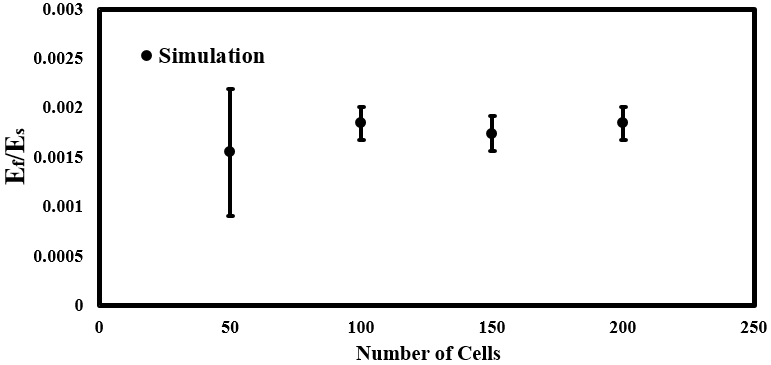
\includegraphics[scale=0.6]{RVEsizeSensitivity}
  \captionsetup{justification=centering}
  \caption[Close up of \textit{Hemidactylus} sp. ]
   {Influence of the number of cells in the RVE on the elastic modulus of the PU foam 
   (normalized by the elastic modulus of the solid PU).}
  \label{fig:RVEsizeSensitivity}
\end{figure}

In addition to the RVE size, the influence of the finite element discretization on the simulation results was assessed in an RVE with 100 cells. Minimum element sizes of 0.02, 0.025, 0.05 and 0.10 mm were chosen and the elastic modulus of the RVE was computed. Similar results were obtained from minimum element sizes of 0.02mm and 0.05 mm and this latter value was used in all the remaining analyses. 

\subsection{Experimental validation}

The numerical predictions for the elastic modulus obtained with an RVE of 100 cells for the 1-3CPW30.2 provided by BASF are shown in Figure~\ref{fig:CalculatedElastic}, together with the experimental values. Numerical simulations were carried out for foams with a density of 30.2 $\mathrm{kg/m^3}$ and cell volume distribution characterized by $\mu=0.39$  and $\sigma=0.15$. In addition, thickness of the faces was varied between 0.15 and 0.7 \SI{}{\micro\metre}. The corresponding fraction of material in the faces varied from 0.05 to 0.23 to assess the influence of the mass in the faces and in the struts on the elastic modulus. Five different realizations were analyzed for each case. The results in Figure~\ref{fig:CalculatedElastic} show very little differences among the five realizations for each material and indicated the elastic modulus increased linearly with the cell thickness. In addition, the simulations carried out assuming a cell thickness of 0.4 \SI{}{\micro\metre} were in excellent agreement with the experimental results. The scanning electron micrographs of the PU foam indicated that the average cell thickness was 0.44 $\pm$ 0.25 \SI{}{\micro\metre}.

\begin{figure}[hb]
  \centering
  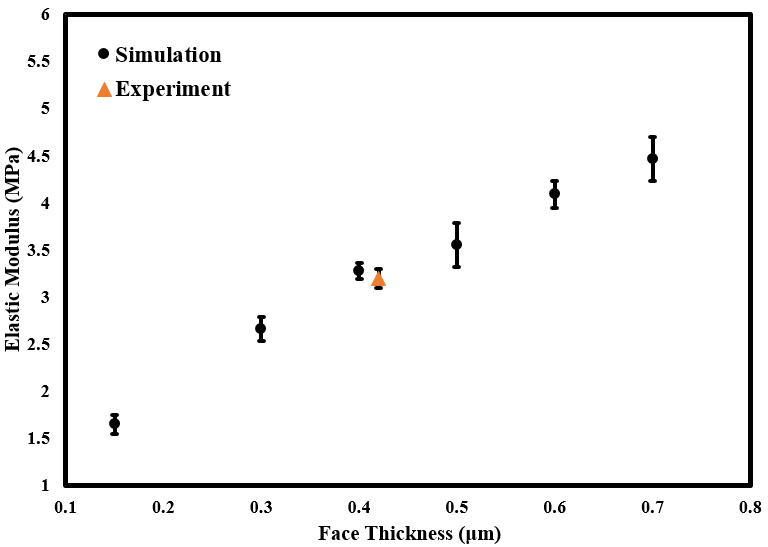
\includegraphics[scale=0.6]{CalculatedElastic}
  \captionsetup{justification=centering}
  \caption[Close up of \textit{Hemidactylus} sp. ]
   {Calculated and measured elastic modulus versus the face thickness.}
  \label{fig:CalculatedElastic}
\end{figure}


Due to the computational instability during the compressive deformation of RVE in high strains (i.e. buckling of shell elements as well as beam elements), FE simulations are performed using explicit analysis to reach the plateau area (10\% strain). The RVE with 100 clles and mesh size of 0.05 is constructed. Since the number of node pairs involved in periodic boundaries are high, using periodic equations offered by ABAQUS is not applicable. As a result, periodic boundary elements are used to tackle this issue \citep{SergioSabadoThesis}. Using periodic boundary elements, one could use periodic boundaries without limitation in number of node pairs. Moreover, based on the experience of the authors, the computational time is much less compared to using ABAQUS periodic boundary equations. 

The representative engineering stress-engineering strain curve of the 1-3CPW- 30.2 foam tested in compression together with FE calculated curves are plotted in Figure~\ref{fig:StressStrainCurveExpFem} (up to 10 percent strain). In order to show the scatter in both experiment and FE results, 3 curves of each are plotted. The FE results show clearly three phenomena as could be seen in experimental results: linear elastic regime, small drop in stress after elastic regime and finally deformation in almost constant stress (plateau stress). Looking more closely to FE results, the observed scatter for plateau stress is higher than the one for stiffness. In other word, the model has more consistency and accuracy in predicting the stiffness rather than the plateau stress, however, experimental results also show more scatter for plateau stress compare to scatter for stiffness. It could have to do with this fact that the stiffness is a demonstration of the average resistance of whole structure under the load and consequently less sensitive to the local phenomena during deformation, while plateau stress is more sensitive to the localized deformation. Moreover, it should bear in mind that the nature of the RVE geometry is random, that for each calculation the new RVE is generated which can have a slightly different total face area (i.e. slightly different shell element thickness, see equation \ref{ThicknessShellElement}) and total length of the struts (i.e. different distribution of material in struts, see equation \ref{TotalLenStruts}). Moreover, the available noise (fluctuation in stress) in calculated (FE) curves could be improved by assigning finer mesh size, that, on the other hand, leads to higher computational cost.

\begin{figure}[hb]
  \centering
  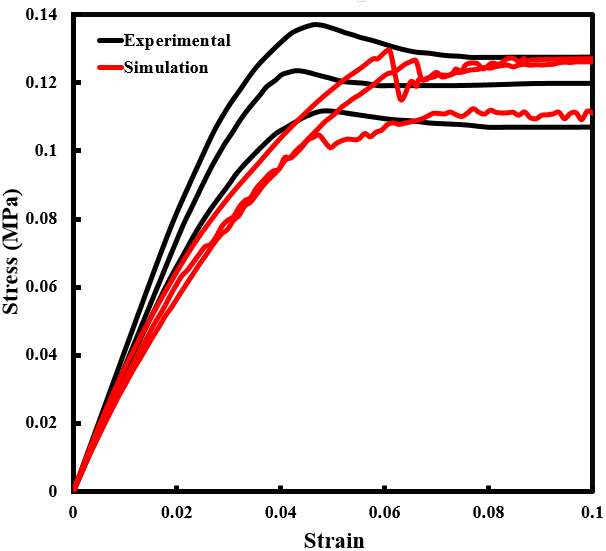
\includegraphics[scale=0.6]{StressStrainCurveExpFem}
  \captionsetup{justification=centering}
  \caption[Close up of \textit{Hemidactylus} sp. ]
   {The engineering stress-engineering strain curve of the 1-3CPW30.2 foam in compression together with FE calculated curves.}
  \label{fig:StressStrainCurveExpFem}
\end{figure} 

\subsection{Deformation mechanism}
As discussed earlier, the model is able to predict three different steps happening till 10\% compressive strain: Linear elastic, slight drop in stress and plateau stress. Since the model consists of two geometric features, struts and faces (beam and shell elements), it is worth reminding that the beam and shell elements have the common nodes in edges, as a result, no separation of faces from struts could be expected in this modelling strategy. However, the acceptable agreement between experimental measurements and FE results (see Figure~\ref{fig:StressStrainCurveExpFem}) shows that the assumption of inseparability of faces from struts does not affect the results significantly. Moreover, as depicted in Figure~\ref{fig:RVEdeformed} (the beam elements are presented with their real cross section as they seem thick in the picture), at high strains close to 10\%, deformation is mainly localized at the top of the RVE, while, at the beginning of deformation it is more uniform throughout the whole structure of the RVE.

\begin{figure}[hb]
  \centering
  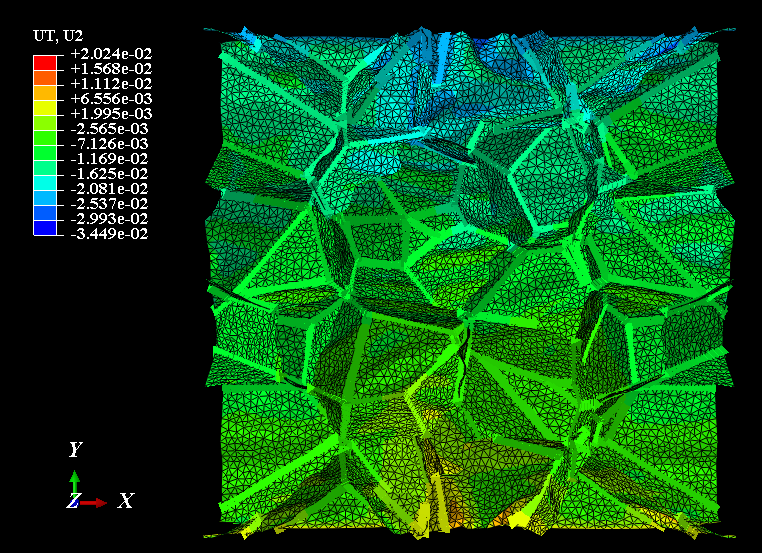
\includegraphics[scale=0.6]{StrainLocalization}
  \captionsetup{justification=centering}
  \caption[Close up of \textit{Hemidactylus} sp. ]
   {The deformed RVE at 10\% strain.}
  \label{fig:RVEdeformed}
\end{figure} 

For the sake of clearance in observing the deformation of faces (shell elements) and struts (beam elements), the cut slice of RVE in $Z$ plane is shown at different levels of strain, figure~\ref{fig:RVEdeformedFaces}. The presented contour showing the nodal axial force (the unit for force is \SI{}{\micro\N}) in both beam and shell elements. Obviously, negative and positive values demonstrating the compressive and tensile loads, respectively. Clearly, during deformation (figure~\ref{fig:RVEdeformedFaces}a to e), the dominant axial load is compressive (negative values). Another point is that, the geometric features, either struts or faces, are showing much higher axial force while located parallel to the loading direction. Moreover, the minimum axial force (negative) and the maximum axial force (positive) happen in struts and faces, respectively; meaning that the faces tolerating tensile loads while struts are under compressive loads.

Apparently, the buckling of faces starts even at the very early stages of loading (see figure~\ref{fig:RVEdeformedFaces}a and b). The early buckling of faces is not surprising, since the volume fraction of solid PU located at the faces is just 15\% results in face thickness of $\approx 0.4$      \SI{}{\micro\metre}, this extremely thin faces could be bent and buckled easily. Moreover, the shell elements at the edges are attached to the beam elements by sharing the nodes. Consequently, it is expected that the faces in the RVE follow the the struts in case of deformation. This is why, as it is for beam elements, the deformation localized at the top of the RVE at high strains figure~\ref{fig:RVEdeformedFaces}e. Although, at the linear elastic step (figure~\ref{fig:RVEdeformedFaces}b), the buckling of faces is uniform in whole structure and can be seen almost in all the faces. In addition, in this step, considering the minimum value for axial force (negative value for the compressive axial load),  the axial force is increasing in RVE by moving toward higher strains. 

Figure~\ref{fig:RVEdeformedFaces}c and d show the state of axial force for all beam and shell elements before and after the small drop in stress of RVE (see figure~\ref{fig:StressStrainCurveExpFem}), respectively. The significant decrease in minimum axial force (from \SI{-3.059e5}{\micro\N} to \SI{-1.442e5}{\micro\N})  explains well the drop in stress. Moreover, the described drop in stress caused by several sequential decrease in axial force. In other words, the buckling of beams located on the struts at the top of the RVE happens step by step and the summation of this successive buckling is a small drop in stress for the RVE. Finally, the minimum axial force shows increasing trend up to 10\%, figure~\ref{fig:RVEdeformedFaces}e. 

 
\begin{figure}[hb]
  \centering
  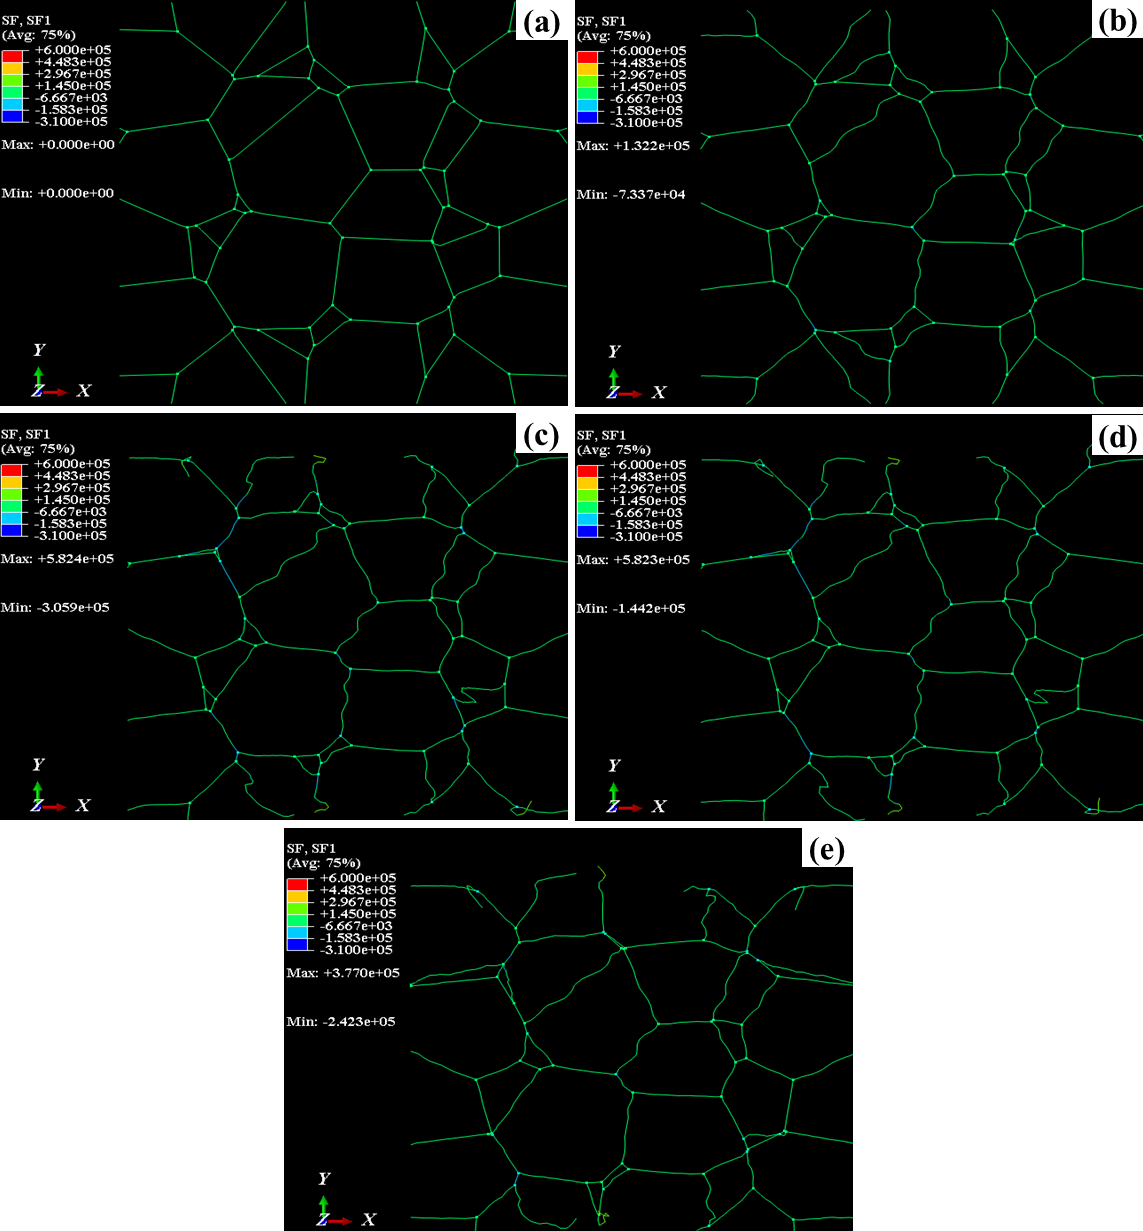
\includegraphics[scale=0.35]{Deformed}
  \captionsetup{justification=centering}
  \caption{Deformed cut of RVE at: (a)0\%, (b)2\%, (c and d)5\%, (e)10\% compressive strain including all beam and shell elements. The loading direction is along $Y$ axis.}
  \label{fig:RVEdeformedFaces}
\end{figure}



????????????'axial force big for struts so they are main load carriiers?????????¿¿¿¿¿¿¿¿¿ interaction of both beam and shells  

\section{Conclusions}
In the current study, modelling strategy to link the geometric features of PU foam, such as cell size distribution, strut shape and strut content, to their mechanical performance under compressive loading was established. In order to build up the RVE as well as validation, one rigid closed-cell PU foam with isotropic geometry was selected as a case study. Through a multiscale characterization procedure (including SEM, XCT and nanoindation), inputs were extracted from the sample in order to build the model and run the simulation. Virtual compression is performed using finite element method, while the struts and faces were modelled with beam and shell elements, respectively. In order to reach high strains while avoiding the computational instabilities could occur due to the buckling of beam and shell elements during analysis, simulations were performed with explicit method. In this case, user defined periodic boundary elements were utilized to apply the compressive loading and increase the model efficiency.

Modelling strategy was validated again the experimental measurement coming from compression test done on the same PU sample. Model with 100 cell is able to predict the stiffness pretty well with an acceptable deviation. On the other hand, prediction of plateau stress showed a bit higher deviation which could source in the random nature of the RVE. Moreover, deformation mechanism was studied in case of three different deformation phenomena observed in compressive stress-strain curve for the PU foam: linear elastic, drop in stress and plateau stress. Trend of compressive axial force in beam and shell elements at the RVE was similar to the trend of engineering stress of the whole RVE. 

Since no plasticity was introduced in the material properties of solid PU in struts and faces, it could be concluded that all non-linearities available in compressive response of PU foam is result of elastic buckling of struts and faces. Although, at the early stages of deformation, bending is the prevailing mechanism, but then the deformation proceeds by sudden buckling of both struts and faces at the top and then buckling phenomenon is distributed uniformly through whole geometry causing constant stress up to large strains. Moreover, if simulation of very high strains (i.e. densification step) is in the area of interest, contact should be introduced to the model as well as gas pressure inside the cells.    


\section*{Acknowledgement}
This study has been founded under the framework of the MODENA project (MOdelling of morphology DEvelopment of micro- and NAnostructures). MoDeNa aims at developing, demonstrating and assessing an easy-to-use multiscale software-modelling framework application under an open-source licensing scheme that delivers models with feasible computational loads for process and product design of complex materials (http://modena.units.it/default.aspx). The scripts developed by authors of current study is available online on https:// github.com/MoDeNa-EUProject/MoDeNa. The authors also would like to appreciate the efforts done by Juraj Kosek research group (Department of Chemical Engineering, ICT Prague) providing some measurements using XCT.


\section*{References}

\bibliography{mybibfile}

\end{document}